\section{ER-діаграма}

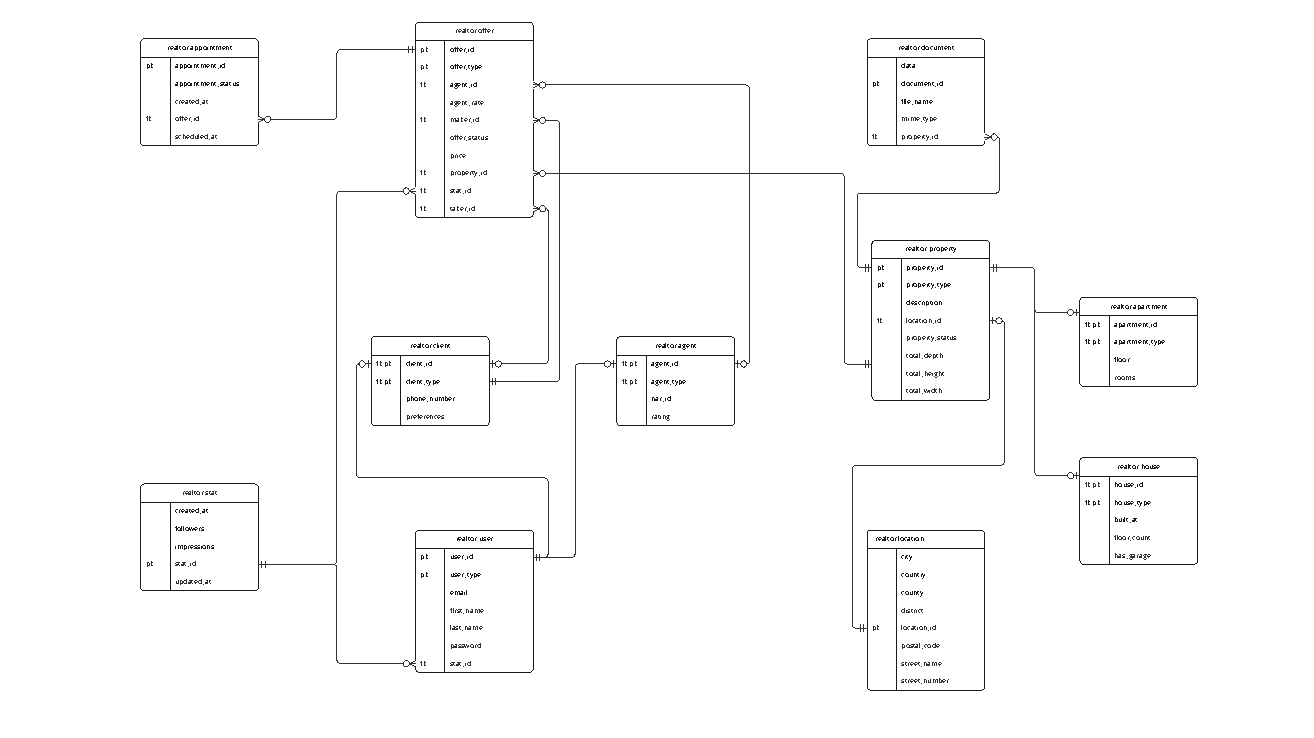
\includegraphics[width=1\linewidth]{../assets/er.pdf}

\section{Зв'язки}

Дизайн Class Table Inheritance є однією з імплементацій паттерну
Generalization/Specialization та використовує зв'язки 0.1-to-1
для імітації наслідування в реляційних базах даних. Його недоліком є
можливість появи осиротілих записів, що потребує додаткових перевірок
використовуючи тригери, двосторонні (deferred) зовнішні ключі,
або періодичний процес їх пошуку та видалення.

\begin{enumerate}
    \item 0.1 agent - 1 user, інакше осиротілий запис
    \item 0.1 apartment - 1 property, інакше осиротілий запис
    \item 0.M appointment - 1 offer
    \item 0.1 client - 1 user, інакше осиротілий запис
    \item 0.M document - 1 property
    \item 0.1 house - 1 property, інакше осиротілий запис
    \item 0.M offer - 0.1 agent
    \item 0.M offer - 1 client
    \item 0.M offer - 0.1 client
    \item 0.M offer - 1 property
    \item 0.M offer - 1 stat
    \item 0.1 property - 1 location
    \item 0.M user - 1 stat
\end{enumerate}
